% The rho of x -> x^2+2 mod 97 from x0=2 (generated by figs_c2ch10.py): tail 2, cycle 8.
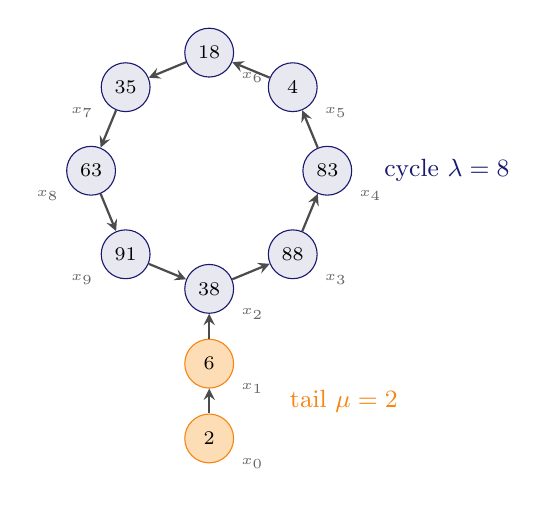
\begin{tikzpicture}[x=1cm,y=1cm,>=stealth]
\tikzset{v/.style={circle,draw=MidnightBlue,fill=MidnightBlue!10,inner sep=1pt,minimum size=0.62cm,font=\scriptsize}}
\node[v,fill=BurntOrange!25,draw=BurntOrange] (r0) at (0.000,0.000) {$2$};
\node[font=\tiny,black!60] at (0.550,-0.320) {$x_{0}$};
\node[v,fill=BurntOrange!25,draw=BurntOrange] (r1) at (0.000,0.950) {$6$};
\node[font=\tiny,black!60] at (0.550,0.630) {$x_{1}$};
\node[v] (r2) at (0.000,1.900) {$38$};
\node[font=\tiny,black!60] at (0.550,1.580) {$x_{2}$};
\node[v] (r3) at (1.061,2.339) {$88$};
\node[font=\tiny,black!60] at (1.611,2.019) {$x_{3}$};
\node[v] (r4) at (1.500,3.400) {$83$};
\node[font=\tiny,black!60] at (2.050,3.080) {$x_{4}$};
\node[v] (r5) at (1.061,4.461) {$4$};
\node[font=\tiny,black!60] at (1.611,4.141) {$x_{5}$};
\node[v] (r6) at (0.000,4.900) {$18$};
\node[font=\tiny,black!60] at (0.550,4.580) {$x_{6}$};
\node[v] (r7) at (-1.061,4.461) {$35$};
\node[font=\tiny,black!60] at (-1.611,4.141) {$x_{7}$};
\node[v] (r8) at (-1.500,3.400) {$63$};
\node[font=\tiny,black!60] at (-2.050,3.080) {$x_{8}$};
\node[v] (r9) at (-1.061,2.339) {$91$};
\node[font=\tiny,black!60] at (-1.611,2.019) {$x_{9}$};
\draw[->,thick,black!70] (r0) -- (r1);
\draw[->,thick,black!70] (r1) -- (r2);
\draw[->,thick,black!70] (r2) -- (r3);
\draw[->,thick,black!70] (r3) -- (r4);
\draw[->,thick,black!70] (r4) -- (r5);
\draw[->,thick,black!70] (r5) -- (r6);
\draw[->,thick,black!70] (r6) -- (r7);
\draw[->,thick,black!70] (r7) -- (r8);
\draw[->,thick,black!70] (r8) -- (r9);
\draw[->,thick,black!70] (r9) -- (r2);
\node[font=\small,BurntOrange,anchor=west] at (0.9,0.475) {tail $\mu=2$};
\node[font=\small,MidnightBlue,anchor=west] at (2.100,3.400) {cycle $\lambda=8$};
\end{tikzpicture}
